\begin{figure*}
\center
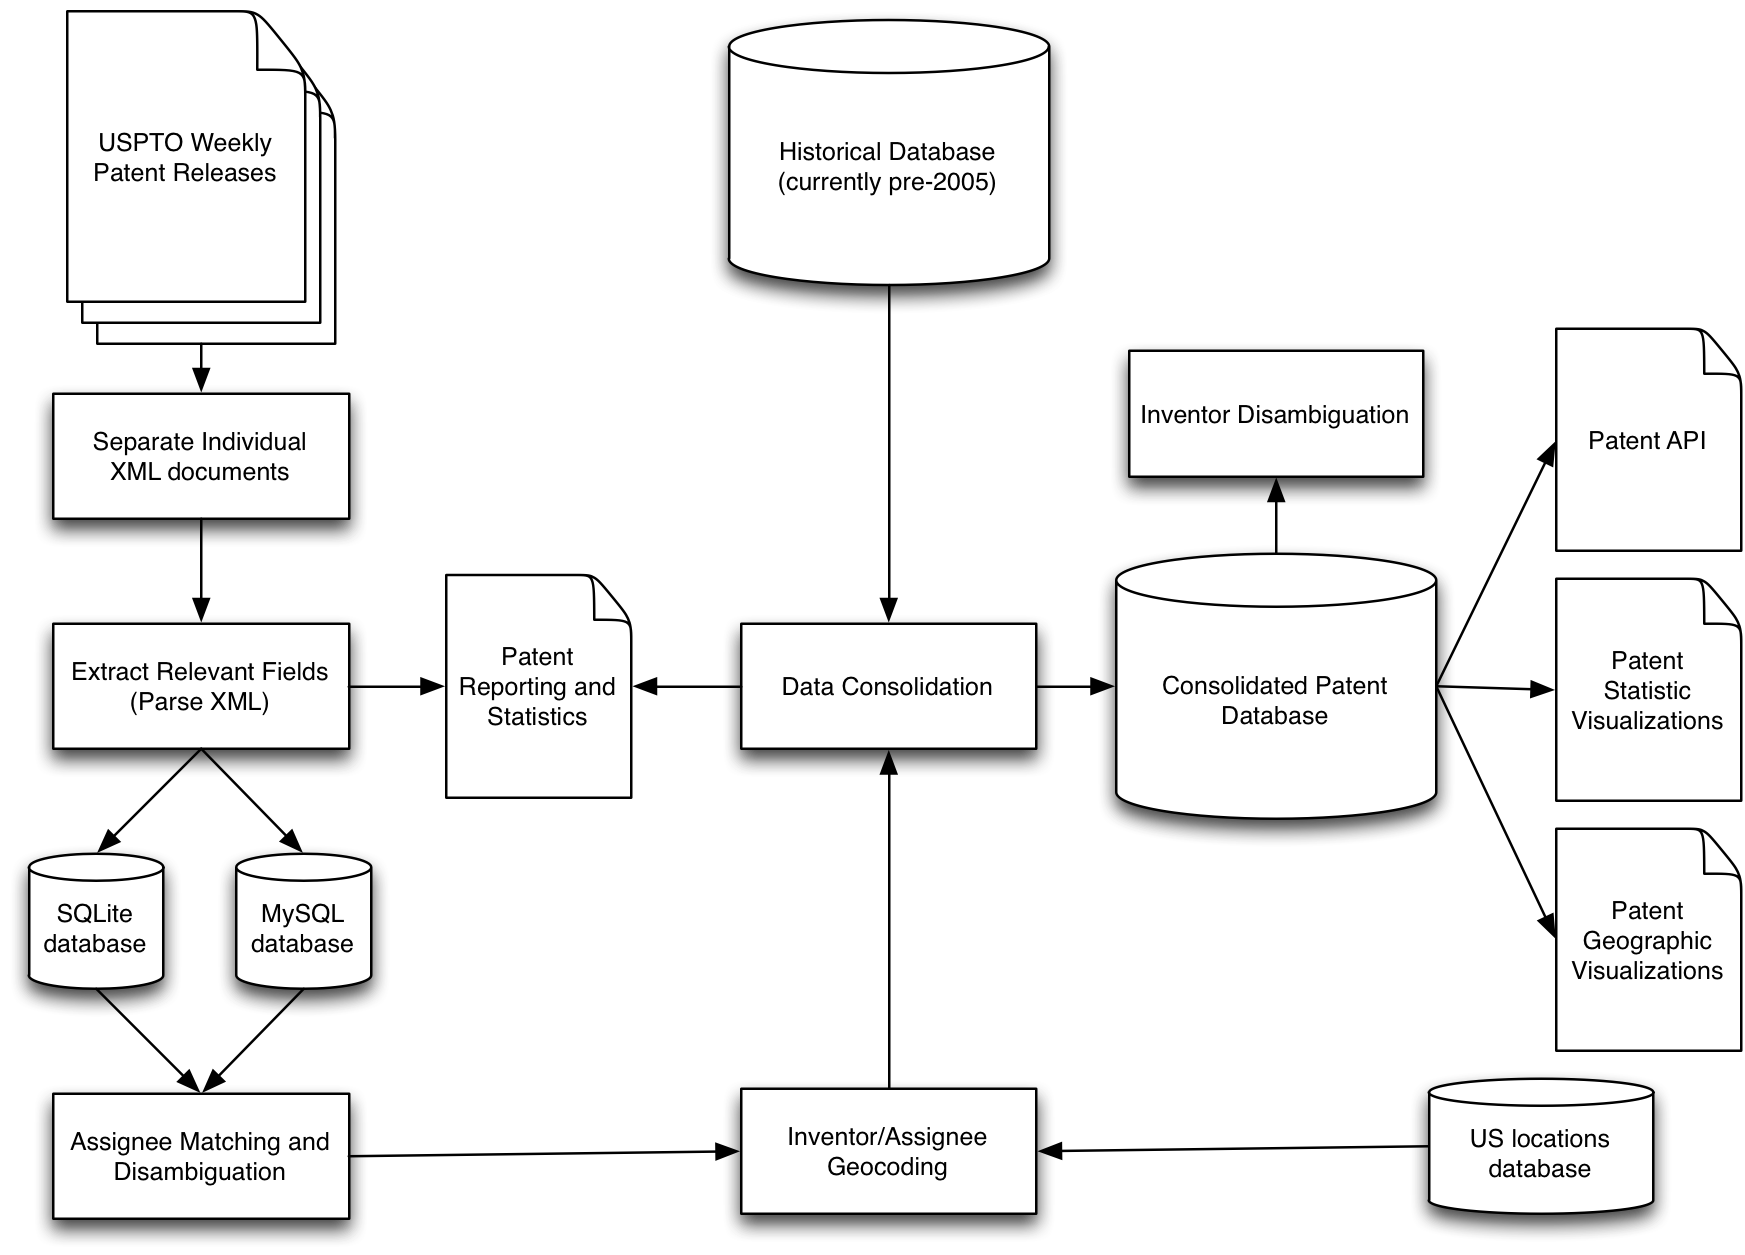
\includegraphics[width=.8\textwidth]{figs/dataprocess}
\caption{Full patent data process flow}
\label{fig:dataprocess}
\end{figure*}

The Fung Institute has developed a robust and fully automated toolchain for processing and providing high quality patent data intended for research, as illustrated in Figure~\ref{fig:dataprocess}.

As data is downloaded from the USPTO weekly patent releases, it is parsed, cleaned and inserted into a SQL database. From this database, assignee and lawyer disambiguations are performed and the patents are geocoded with a location-based disambiguation. The output data from these processes are combined with the historical data from the Harvard Dataverse Network into a single consolidated database. From this database, an inventor-level disambiguation can be performed, and various applications can take advantage of the completed data.